% answers.tex —— 2008 年·普通高等学校招生考试·上海卷·文科 · 参考答案与详细解析片段
% 由 tools/generate_projects.py 依来源总账自 2008/2008_数学真题_上海文_试题.md + 2008/2008_数学真题_上海文_解析正文.md + 2008/2008_数学真题_上海文_答案要点.md 生成，勿手改（改源 MD 后重跑）


\begin{gktip}
固定候选 PDF 仅含题面，无答案、解析和评分标准，原卷亦未标注分值；以下为非官方编者独立推导，官方答案字段为空。来源发布者、出版者、版次与官方身份均未核。
\end{gktip}

\begin{answer}
\gksolhead{1}{}

\textbf{题目}：

不等式 $|x-1|<1$ 的解集是\gkblank{}。

\Needspace{4\baselineskip}
\textbf{解析}

\Needspace{5\baselineskip}
计算如下：

\nopagebreak[4]
\[|x-1|<1\ \Longleftrightarrow\ -1<x-1<1\ \Longleftrightarrow\ 0<x<2.\]

\gkanswer{答案：$(0,2)$。}

\end{answer}
\begin{answer}
\gksolhead{2}{}

\textbf{题目}：

若集合 $A=\{x\mid x\leqslant2\}$，$B=\{x\mid x\geqslant a\}$ 满足 $A\cap B=\{2\}$，则实数 $a=$\gkblank{}。

\Needspace{4\baselineskip}
\textbf{解析}

\Needspace{5\baselineskip}
$A=(-\infty,2]$，$B=[a,+\infty)$，故

\nopagebreak[4]
\[A\cap B=[a,2].\]

要使 $A\cap B=\{2\}$，需 $a=2$。

\gkanswer{答案：$2$。}

\end{answer}
\begin{answer}
\gksolhead{3}{}

\textbf{题目}：

若复数 $z$ 满足 $z=\mathrm i(2-z)$（$\mathrm i$ 是虚数单位），则 $z=$\gkblank{}。

\Needspace{4\baselineskip}
\textbf{解析}

\Needspace{5\baselineskip}
由 $z=\mathrm i(2-z)$ 得

\nopagebreak[4]
\[z(1+\mathrm i)=2\mathrm i,\qquad z=\frac{2\mathrm i}{1+\mathrm i}=\frac{2\mathrm i(1-\mathrm i)}2=\mathrm i(1-\mathrm i)=1+\mathrm i.\]

\gkanswer{答案：$1+\mathrm i$。}

\end{answer}
\begin{answer}
\gksolhead{4}{}

\textbf{题目}：

若函数 $f(x)$ 的反函数为 $f^{-1}(x)=\log_2x$，则 $f(x)=$\gkblank{}。

\Needspace{4\baselineskip}
\textbf{解析}

$f^{-1}(x)=\log_2x$ 的反函数为 $f(x)=2^x$。

\gkanswer{答案：$2^x$。}

\end{answer}
\begin{answer}
\gksolhead{5}{}

\textbf{题目}：

若向量 $\boldsymbol a$，$\boldsymbol b$ 满足 $|\boldsymbol a|=1$，$|\boldsymbol b|=2$，且 $\boldsymbol a$ 与 $\boldsymbol b$ 的夹角为 $\dfrac{\pi}3$，则 $|\boldsymbol a+\boldsymbol b|=$\gkblank{}。

\Needspace{4\baselineskip}
\textbf{解析}

\Needspace{5\baselineskip}
计算如下：

\nopagebreak[4]
\[|\boldsymbol a+\boldsymbol b|^2=|\boldsymbol a|^2+|\boldsymbol b|^2+2\boldsymbol a\cdot\boldsymbol b=1+4+2\times1\times2\cos\frac{\pi}3=5+2=7,\]

故 $|\boldsymbol a+\boldsymbol b|=\sqrt7$。

\gkanswer{答案：$\sqrt7$。}

\end{answer}
\begin{answer}
\gksolhead{6}{}

\textbf{题目}：

若直线 $ax-y+1=0$ 经过抛物线 $y^2=4x$ 的焦点，则实数 $a=$\gkblank{}。

\Needspace{4\baselineskip}
\textbf{解析}

\Needspace{5\baselineskip}
抛物线 $y^2=4x$ 的焦点为 $(1,0)$。代入 $ax-y+1=0$：

\nopagebreak[4]
\[a+1=0,\qquad a=-1.\]

\gkanswer{答案：$-1$。}

\end{answer}
\begin{answer}
\gksolhead{7}{}

\textbf{题目}：

若 $z$ 是实系数方程 $x^2+2x+p=0$ 的一个虚根，且 $|z|=2$，则 $p=$\gkblank{}。

\Needspace{4\baselineskip}
\textbf{解析}

\Needspace{5\baselineskip}
实系数方程的虚根成共轭出现，设 $z$，$\bar z$ 为两根，则

\nopagebreak[4]
\[z\bar z=|z|^2=p.\]

由 $|z|=2$ 得 $p=4$。

\gkanswer{答案：$4$。}

\end{answer}
\begin{answer}
\gksolhead{8}{}

\textbf{题目}：

在平面直角坐标系中，从五个点 $A(0,0)$，$B(2,0)$，$C(1,1)$，$D(0,2)$，$E(2,2)$ 中任取三个，这三点能构成三角形的概率是\gkblank{}。（结果用分数表示）

\Needspace{4\baselineskip}
\textbf{解析}

\Needspace{5\baselineskip}
任取三点共 $\mathrm C_5^3=10$ 种。三点共线的情形：

\nopagebreak[4]
\[A(0,0),\ C(1,1),\ E(2,2)\quad\text{\text{共线}};\qquad B(2,0),\ C(1,1),\ D(0,2)\quad\text{\text{共线}},\]

\Needspace{5\baselineskip}
共 $2$ 种，故能构成三角形的概率为

\nopagebreak[4]
\[\frac{10-2}{10}=\frac45.\]

\gkanswer{答案：$\dfrac45$。}

\end{answer}
\begin{answer}
\gksolhead{9}{}

\textbf{题目}：

若函数 $f(x)=(x+a)(bx+2a)$（常数 $a$，$b\in\mathbf R$）是偶函数，且它的值域为 $(-\infty,4]$，则该函数的解析式 $f(x)=$\gkblank{}。

\Needspace{4\baselineskip}
\textbf{解析}

\Needspace{5\baselineskip}
计算如下：

\nopagebreak[4]
\[f(x)=bx^2+(2a+ab)x+2a^2.\]

\Needspace{5\baselineskip}
$f$ 为偶函数，一次项系数为零：

\nopagebreak[4]
\[a(2+b)=0.\]

\Needspace{5\baselineskip}
若 $a=0$，则 $f(x)=0$，值域为 $\{0\}$，不合题意，故 $b=-2$。此时

\nopagebreak[4]
\[f(x)=-2x^2+2a^2,\]

\Needspace{5\baselineskip}
值域为 $(-\infty,2a^2]$。由 $2a^2=4$ 得 $a^2=2$，故

\nopagebreak[4]
\[f(x)=-2x^2+4.\]

\gkanswer{答案：$-2x^2+4$。}

\end{answer}
\begin{answer}
\gksolhead{10}{}

\textbf{题目}：

已知总体的各个体的值由小到大依次为 $2$，$3$，$3$，$7$，$a$，$b$，$12$，$13.7$，$18.3$，$20$，且总体的中位数为 $10.5$。若要使该总体的方差最小，则 $a$，$b$ 的取值分别是\gkblank{}。

\Needspace{4\baselineskip}
\textbf{解析}

\Needspace{5\baselineskip}
由中位数为 $10.5$：

\nopagebreak[4]
\[\frac{a+b}2=10.5,\qquad a+b=21.\]

\Needspace{5\baselineskip}
总体均值

\nopagebreak[4]
\[\bar x=\frac{2+3+3+7+a+b+12+13.7+18.3+20}{10}=\frac{79+21}{10}=10.\]

\Needspace{5\baselineskip}
方差最小时 $a$，$b$ 应尽量接近均值 $10$；结合 $a+b=21$ 且 $7\leqslant a\leqslant b\leqslant12$，取

\nopagebreak[4]
\[a=10,\qquad b=11.\]

\gkanswer{答案：$a=10$，$b=11$。}

\end{answer}
\begin{answer}
\gksolhead{11}{}

\textbf{题目}：

在平面直角坐标系中，点 $A$，$B$，$C$ 的坐标分别为 $(0,1)$，$(4,2)$，$(2,6)$。如果 $P(x,y)$ 是 $\triangle ABC$ 围成的区域（含边界）上的点，那么当 $w=xy$ 取到最大值时，点 $P$ 的坐标是\gkblank{}。

\Needspace{4\baselineskip}
\textbf{解析}

边界上逐段考察 $w=xy$：

$AB$：$y=1+\dfrac x4$（$0\leqslant x\leqslant4$），$w=x+\dfrac{x^2}4$ 递增，最大值在 $B$ 处为 $8$。

$AC$：$y=1+\dfrac52x$（$0\leqslant x\leqslant2$），$w=x+\dfrac52x^2$ 递增，最大值在 $C$ 处为 $12$。

\Needspace{5\baselineskip}
$BC$：$y=10-2x$（$2\leqslant x\leqslant4$），

\nopagebreak[4]
\[w=x(10-2x)=-2x^2+10x,\]

\Needspace{5\baselineskip}
在 $x=\dfrac52$ 处取最大值

\nopagebreak[4]
\[w=-2\cdot\frac{25}4+25=\frac{25}2,\]

此时 $y=10-5=5$。故 $P\left(\dfrac52,5\right)$。

\gkanswer{答案：$\left(\dfrac52,5\right)$。}

\end{answer}
\begin{answer}
\gksolhead{12}{}

\textbf{题目}：

设 $P$ 是椭圆 $\dfrac{x^2}{25}+\dfrac{y^2}{16}=1$ 上的点。若 $F_1$，$F_2$ 是椭圆的两个焦点，则 $|PF_1|+|PF_2|$ 等于（　）

（A）$4$

（B）$5$

（C）$8$

（D）$10$

\Needspace{4\baselineskip}
\textbf{解析}

\Needspace{5\baselineskip}
椭圆中 $a^2=25$，$a=5$，由椭圆定义

\nopagebreak[4]
\[|PF_1|+|PF_2|=2a=10.\]

\gkanswer{答案：D。}

\end{answer}
\begin{answer}
\gksolhead{13}{}

\textbf{题目}：

给定空间中的直线 $l$ 及平面 $\alpha$，条件“直线 $l$ 与平面 $\alpha$ 内无数条直线都垂直”是“直线 $l$ 与平面 $\alpha$ 垂直”的（　）

（A）充分非必要条件

（B）必要非充分条件

（C）充要条件

（D）既非充分又非必要条件

\Needspace{4\baselineskip}
\textbf{解析}

若 $l\perp\alpha$，则 $l$ 垂直于 $\alpha$ 内所有直线，必垂直于无数条，必要性成立。

反之，$l$ 只需垂直于 $\alpha$ 内一组平行直线即可垂直于“无数条”直线，未必垂直于 $\alpha$，充分性不成立。

\gkanswer{答案：B。}

\end{answer}
\begin{answer}
\gksolhead{14}{}

\textbf{题目}：

若数列 $\{a_n\}$ 是首项为 $1$，公比为 $a-\dfrac32$ 的无穷等比数列，且 $\{a_n\}$ 各项的和为 $a$，则 $a$ 的值是（　）

（A）$1$

（B）$2$

（C）$\dfrac12$

（D）$\dfrac54$

\Needspace{4\baselineskip}
\textbf{解析}

\Needspace{5\baselineskip}
无穷等比数列各项和

\nopagebreak[4]
\[S=\frac1{1-q}=a,\qquad q=a-\frac32,\]

\Needspace{5\baselineskip}
故

\nopagebreak[4]
\[1=a\left(1-a+\frac32\right)=a\left(\frac52-a\right),\]

\nopagebreak[4]
\[2a^2-5a+2=0,\qquad a=2\ \text{\text{或}}\ a=\frac12.\]

收敛要求 $|q|<1$：$a=2$ 时 $q=\dfrac12$ 符合；$a=\dfrac12$ 时 $q=-1$，不符合。故 $a=2$。

\gkanswer{答案：B。}

\end{answer}
\begin{answer}
\gksolhead{15}{}

\textbf{题目}：

如图，在平面直角坐标系中，$\Omega$ 是一个与 $x$ 轴的正半轴、$y$ 轴的正半轴分别相切于点 $C$、$D$ 的定圆所围成区域（含边界），$A$、$B$、$C$、$D$ 是该圆的四等分点。若点 $P(x,y)$、点 $P'(x',y')$ 满足 $x\leqslant x'$ 且 $y\geqslant y'$，则称 $P$ 优于 $P'$。如果 $\Omega$ 中的点 $Q$ 满足：不存在 $\Omega$ 中的其它点优于 $Q$，那么所有这样的点 $Q$ 组成的集合是劣弧（　）
\nopagebreak[4]
\begin{center}% 2008 年上海卷文科第 15 题：圆 Ω 与 x、y 轴正半轴分别切于 C、D，
%   A、B、C、D 为圆的四等分点（A 上、B 右、C 下、D 左）。
% 来源 PDF：gaokaomath-src/普通高考/2008/2008上海文.pdf
% SHA-256：415d384fcd05cab11debea2d8a328f9daf1d1880ffd26c915df999f7bae589a4
% 原页：2008上海文.pdf 第 1 页（A3 三栏）第 2 栏，书页码 481。
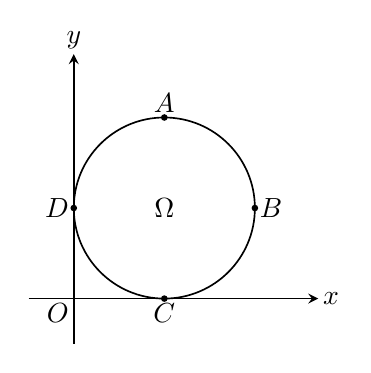
\begin{tikzpicture}[x=1.15cm, y=1.15cm, semithick,
  every node/.style={inner sep=1.5pt}]
  \draw[->,>=stealth] (-0.5,0) -- (2.7,0) node[right] {$x$};
  \draw[->,>=stealth] (0,-0.5) -- (0,2.7) node[above] {$y$};
  \node[below left] at (0,0) {$O$};
  \draw (1,1) circle (1);
  \node at (1,1) {$\Omega$};
  \fill (1,2) circle (1.2pt); \node[above] at (1,2) {$A$};
  \fill (2,1) circle (1.2pt); \node[right] at (2,1) {$B$};
  \fill (1,0) circle (1.2pt); \node[below] at (1,0) {$C$};
  \fill (0,1) circle (1.2pt); \node[left] at (0,1) {$D$};
\end{tikzpicture}
\end{center}
\nopagebreak[4]
（A）$\widehat{AB}$

（B）$\widehat{BC}$

（C）$\widehat{CD}$

（D）$\widehat{DA}$

\Needspace{4\baselineskip}
\textbf{解析}

“$P$ 优于 $P'$” 即 $P$ 在 $P'$ 的左侧且不低。要被优于，需存在 $\Omega$ 内一点横坐标更小、纵坐标更大。

圆与两轴相切，圆心 $(r,r)$，$A(r,2r)$，$B(2r,r)$，$C(r,0)$，$D(0,r)$。对弧 $\widehat{DA}$ 上的点 $Q$，$\Omega$ 内横坐标不超过 $Q$ 的点都在 $Q$ 的右下方（或就是 $Q$），不存在优于 $Q$ 的点；而弧 $\widehat{AB}$、$\widehat{BC}$、$\widehat{CD}$ 上的点都可被更左更上的点优于（如 $A$、$D$）。故所求集合是 $\widehat{DA}$。

\gkanswer{答案：D。}

\end{answer}
\begin{answer}
\gksolhead{16}{}

\textbf{题目}：

如图，在棱长为 $2$ 的正方体 $ABCD-A_1B_1C_1D_1$ 中，$E$ 是 $BC_1$ 的中点。求直线 $DE$ 与平面 $ABCD$ 所成角的大小。（结果用反三角函数表示）
\nopagebreak[4]
\begin{center}% 2008 年上海卷文科第 16 题：棱长 2 的正方体 ABCD-A1B1C1D1，E 为 BC1 的中点，
%   求直线 DE 与平面 ABCD 所成的角。
% 来源 PDF：gaokaomath-src/普通高考/2008/2008上海文.pdf
% SHA-256：415d384fcd05cab11debea2d8a328f9daf1d1880ffd26c915df999f7bae589a4
% 原页：2008上海文.pdf 第 1 页（A3 三栏）第 2 栏，书页码 481。
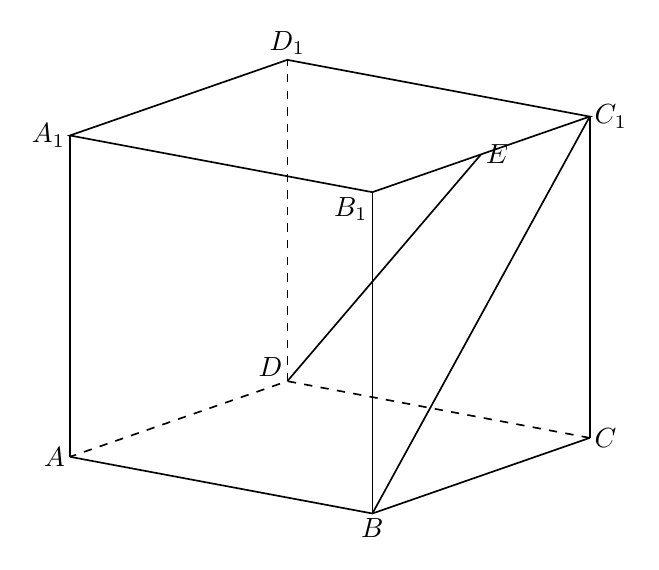
\begin{tikzpicture}[scale=1.2, semithick,
  every node/.style={inner sep=1.5pt}]
  \coordinate (A)  at (0.0,0.9);
  \coordinate (B)  at (3.2,0.3);
  \coordinate (C)  at (5.5,1.1);
  \coordinate (D)  at (2.3,1.7);
  \coordinate (A1) at (0.0,4.3);
  \coordinate (B1) at (3.2,3.7);
  \coordinate (C1) at (5.5,4.5);
  \coordinate (D1) at (2.3,5.1);
  \coordinate (E)  at (4.35,4.1);

  \draw (A) -- (B) -- (C);
  \draw[dashed] (C) -- (D) -- (A);
  \draw (A) -- (A1);
  \draw (B) -- (B1);
  \draw (C) -- (C1);
  \draw (D1) -- (A1) -- (B1) -- (C1) -- cycle;
  \draw[dashed] (D) -- (D1);

  \draw (D) -- (E);
  \draw (B) -- (C1);

  \node[left] at (A) {$A$};
  \node[below] at (B) {$B$};
  \node[right] at (C) {$C$};
  \node[above left] at (D) {$D$};
  \node[left] at (A1) {$A_1$};
  \node[below left] at (B1) {$B_1$};
  \node[right] at (C1) {$C_1$};
  \node[above] at (D1) {$D_1$};
  \node[right] at (E) {$E$};
\end{tikzpicture}
\end{center}
\nopagebreak[4]
\Needspace{4\baselineskip}
\textbf{解析}

\Needspace{5\baselineskip}
以 $A$ 为原点，$AB$，$AD$，$AA_1$ 为 $x$，$y$，$z$ 轴，取

\nopagebreak[4]
\[D(0,2,0),\quad B(2,0,0),\quad C_1(2,2,2),\quad E(2,1,1).\]

\nopagebreak[4]
\[\overrightarrow{DE}=(2,-1,1).\]

\Needspace{5\baselineskip}
平面 $ABCD$ 的法向量为 $(0,0,1)$。设所求角为 $\theta$：

\nopagebreak[4]
\[\sin\theta=\frac{1}{\sqrt{2^2+(-1)^2+1^2}}=\frac1{\sqrt6}=\frac{\sqrt6}6,\]

故 $\theta=\arcsin\dfrac{\sqrt6}6$。

\gkanswer{答案：$\arcsin\dfrac{\sqrt6}6$。}

\end{answer}
\begin{answer}
\gksolhead{17}{}

\textbf{题目}：

如图，某住宅小区的平面图呈扇形 $AOC$。小区的两个出入口设置在点 $A$ 及点 $C$ 处，小区里有两条笔直的小路 $AD$、$DC$，且拐弯处的转角为 $120^\circ$。已知某人从 $C$ 沿 $CD$ 走到 $D$ 用了 $10$ 分钟，从 $D$ 沿 $DA$ 走到 $A$ 用了 $6$ 分钟。若此人步行的速度为每分钟 $50$ 米，求该扇形的半径 $OA$ 的长。（精确到 $1$ 米）
\nopagebreak[4]
\begin{center}% 2008 年上海卷文科第 17 题：扇形 AOC，出入口在 A、C，内部小路 AD、DC，
%   拐弯处 D 的转角为 120°，CD=500 m，DA=300 m。
% 来源 PDF：gaokaomath-src/普通高考/2008/2008上海文.pdf
% SHA-256：415d384fcd05cab11debea2d8a328f9daf1d1880ffd26c915df999f7bae589a4
% 原页：2008上海文.pdf 第 1 页（A3 三栏）第 3 栏，书页码 481。
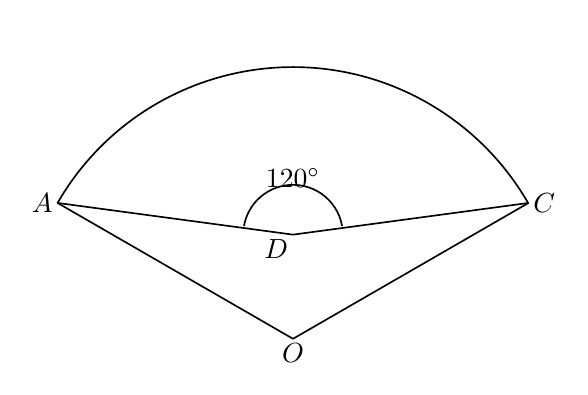
\begin{tikzpicture}[scale=1.15, semithick,
  every node/.style={inner sep=1.5pt}]
  \coordinate (O) at (0,0);
  \coordinate (A) at (-2.6,1.5);
  \coordinate (C) at (2.6,1.5);
  \coordinate (D) at (0,1.15);

  % 扇形弧
  \draw (A) arc[start angle=150, end angle=30, radius=3.0];
  \draw (O) -- (A);
  \draw (O) -- (C);

  % 小路
  \draw (A) -- (D) -- (C);

  % 转角
  \draw (D) ++(10:0.55) arc[start angle=10, end angle=170, radius=0.55];
  \node at (0,1.78) {$120^\circ$};

  \node[left] at (A) {$A$};
  \node[right] at (C) {$C$};
  \node[below left] at (D) {$D$};
  \node[below] at (O) {$O$};
\end{tikzpicture}
\end{center}
\nopagebreak[4]
\Needspace{4\baselineskip}
\textbf{解析}

\Needspace{5\baselineskip}
计算如下：

\nopagebreak[4]
\[CD=50\times10=500\ (\text{\text{米}}),\qquad DA=50\times6=300\ (\text{\text{米}}).\]

\Needspace{5\baselineskip}
在 $\triangle ADC$ 中，$\angle ADC=120^\circ$，由余弦定理

\nopagebreak[4]
\[AC^2=500^2+300^2-2\times500\times300\cos120^\circ=250000+90000+150000=490000,\]

故 $AC=700$。

\Needspace{5\baselineskip}
由图形，扇形圆心角 $\angle AOC=120^\circ$（原页文字未另给此角，见下方源疑点）。于是

\nopagebreak[4]
\[AC=2R\sin60^\circ,\qquad R=\frac{700}{\sqrt3}=\frac{700\sqrt3}3\approx404.1.\]

精确到 $1$ 米，半径 $OA\approx404$ 米。

【源疑点：原页文字只说“扇形 $AOC$”，没有给出圆心角；图中 $D$ 画在扇形内部，$AD$、$DC$、$\angle ADC$ 三条件本身不足以确定半径。按图形（$\angle AOC=120^\circ$）与“精确到 1 米”的答案口径，取圆心角 $120^\circ$，得 $404$ 米。】

\gkanswer{答案：约 $404$ 米。}

\end{answer}
\begin{answer}
\gksolhead{18}{}

\textbf{题目}：

已知函数 $f(x)=\sin2x$，$g(x)=\cos\left(2x+\dfrac{\pi}6\right)$，直线 $x=t$（$t\in\mathbf R$）与函数 $f(x)$、$g(x)$ 的图象分别交于 $M$、$N$ 两点。

（1）当 $t=\dfrac{\pi}4$ 时，求 $|MN|$ 的值；

（2）求 $|MN|$ 在 $t\in\left[0,\dfrac{\pi}2\right]$ 时的最大值。

\Needspace{4\baselineskip}
\textbf{解析}

\Needspace{5\baselineskip}
（1）$t=\dfrac{\pi}4$ 时，

\nopagebreak[4]
\[f\left(\frac{\pi}4\right)=\sin\frac{\pi}2=1,\qquad g\left(\frac{\pi}4\right)=\cos\left(\frac{\pi}2+\frac{\pi}6\right)=\cos\frac{2\pi}3=-\frac12,\]

故 $|MN|=\left|1-\left(-\dfrac12\right)\right|=\dfrac32$。

\Needspace{5\baselineskip}
（2）

\nopagebreak[4]
\[f(t)-g(t)=\sin2t-\cos\left(2t+\frac{\pi}6\right)
=\sin2t-\left(\frac{\sqrt3}2\cos2t-\frac12\sin2t\right)
=\frac32\sin2t-\frac{\sqrt3}2\cos2t.\]

\Needspace{5\baselineskip}
再化为

\nopagebreak[4]
\[f(t)-g(t)=\sqrt3\sin\left(2t-\frac{\pi}6\right).\]

\Needspace{5\baselineskip}
当 $t\in\left[0,\dfrac{\pi}2\right]$ 时，$2t-\dfrac{\pi}6\in\left[-\dfrac{\pi}6,\dfrac{5\pi}6\right]$，$\sin\left(2t-\dfrac{\pi}6\right)$ 可取到 $1$（$t=\dfrac{\pi}3$），故

\nopagebreak[4]
\[|MN|_{\max}=\sqrt3.\]

\gkanswer{答案：（1）$\dfrac32$；（2）$\sqrt3$。}

\end{answer}
\begin{answer}
\gksolhead{19}{}

\textbf{题目}：

已知函数 $f(x)=2^x-\dfrac1{2^{|x|}}$。

（1）若 $f(x)=2$，求 $x$ 的值；

（2）若 $2^tf(2t)+mf(t)\geqslant0$ 对于 $t\in[1,2]$ 恒成立，求实数 $m$ 的取值范围。

\Needspace{4\baselineskip}
\textbf{解析}

\Needspace{5\baselineskip}
（1）若 $x\geqslant0$，

\nopagebreak[4]
\[2^x-2^{-x}=2\ \Longrightarrow\ (2^x)^2-2\cdot2^x-1=0\ \Longrightarrow\ 2^x=1+\sqrt2,\]

\nopagebreak[4]
\[x=\log_2(1+\sqrt2).\]

若 $x<0$，则 $2^x-2^{x}=0\neq2$，无解。

\Needspace{5\baselineskip}
（2）$t\in[1,2]$ 时 $t>0$，

\nopagebreak[4]
\[f(t)=2^t-2^{-t},\qquad f(2t)=2^{2t}-2^{-2t},\]

\nopagebreak[4]
\[2^tf(2t)+mf(t)=2^{3t}-2^{-t}+m\left(2^t-2^{-t}\right).\]

\Needspace{5\baselineskip}
令 $u=2^t\in[2,4]$，则 $2^{3t}=u^3$，$2^{-t}=\dfrac1u$，不等式化为

\nopagebreak[4]
\[u^3-\frac1u+m\left(u-\frac1u\right)\geqslant0.\]

\Needspace{5\baselineskip}
两边乘 $u>0$：

\nopagebreak[4]
\[u^4-1+m(u^2-1)\geqslant0
\ \Longleftrightarrow\ (u^2-1)(u^2+1+m)\geqslant0.\]

\Needspace{5\baselineskip}
$u\in[2,4]$ 时 $u^2-1>0$，故需

\nopagebreak[4]
\[u^2+1+m\geqslant0\]

\Needspace{5\baselineskip}
对 $u\in[2,4]$ 恒成立，即

\nopagebreak[4]
\[m\geqslant-\left(u^2+1\right)_{\max}=-(2^2+1)=-5.\]

\gkanswer{答案：（1）$\log_2(1+\sqrt2)$；（2）$m\geqslant-5$。}

\end{answer}
\begin{answer}
\gksolhead{20}{}

\textbf{题目}：

已知双曲线 $C:\dfrac{x^2}2-y^2=1$。

（1）求双曲线 $C$ 的渐近线方程；

（2）已知点 $M$ 的坐标为 $(0,1)$。设 $P$ 是双曲线 $C$ 上的点，$Q$ 是点 $P$ 关于原点的对称点。记 $\lambda=\overrightarrow{MP}\cdot\overrightarrow{MQ}$，求 $\lambda$ 的取值范围；

（3）已知点 $D$、$E$、$M$ 的坐标分别为 $(-2,-1)$、$(2,-1)$、$(0,1)$，$P$ 为双曲线 $C$ 上在第一象限内的点。记 $l$ 为经过原点与点 $P$ 的直线，$s$ 为 $\triangle DEM$ 截直线 $l$ 所得线段的长。试将 $s$ 表示为直线 $l$ 的斜率 $k$ 的函数。

\Needspace{4\baselineskip}
\textbf{解析}

\Needspace{5\baselineskip}
（1）令 $\dfrac{x^2}2-y^2=0$，得渐近线

\nopagebreak[4]
\[y=\pm\frac{\sqrt2}2x.\]

\Needspace{5\baselineskip}
（2）设 $P(x,y)$ 在 $C$ 上，则 $Q(-x,-y)$，

\nopagebreak[4]
\[\lambda=\overrightarrow{MP}\cdot\overrightarrow{MQ}=(x,y-1)\cdot(-x,-y-1)=-x^2-y^2+1.\]

\Needspace{5\baselineskip}
由 $x^2=2+2y^2$ 得

\nopagebreak[4]
\[\lambda=-(2+2y^2)-y^2+1=-3y^2-1\leqslant-1,\]

且 $y$ 可取任意实数，故 $\lambda\in(-\infty,-1]$。

\Needspace{5\baselineskip}
（3）设 $l:y=kx$。$P$ 在第一象限，$k>0$；由 $x^2\left(\dfrac12-k^2\right)=1$ 需

\nopagebreak[4]
\[0<k<\frac{\sqrt2}2.\]

$\triangle DEM$ 的三边：$DE:y=-1$（$-2\leqslant x\leqslant2$），$DM:y=x+1$（$-2\leqslant x\leqslant0$），$EM:y=-x+1$（$0\leqslant x\leqslant2$）。

\Needspace{5\baselineskip}
当 $0<k\leqslant\dfrac12$ 时，$l$ 与 $DM$ 交于 $x=\dfrac1{k-1}$（$\in[-2,0)$），与 $EM$ 交于 $x=\dfrac1{k+1}$，故

\nopagebreak[4]
\[s=\sqrt{1+k^2}\left(\frac1{k+1}-\frac1{k-1}\right)=\frac{2\sqrt{1+k^2}}{1-k^2}.\]

\Needspace{5\baselineskip}
当 $\dfrac12<k<\dfrac{\sqrt2}2$ 时，$l$ 与 $DE$ 交于 $\left(-\dfrac1k,-1\right)$，与 $EM$ 交于 $x=\dfrac1{k+1}$，故

\nopagebreak[4]
\[s=\sqrt{1+k^2}\left(\frac1{k+1}+\frac1k\right)=\frac{(2k+1)\sqrt{1+k^2}}{k(k+1)}.\]

两段在 $k=\dfrac12$ 处都给出 $s=\dfrac{4\sqrt5}3$，衔接。

\gkanswer{答案：（1）$y=\pm\dfrac{\sqrt2}2x$；（2）$(-\infty,-1]$；（3）分段函数见解析。}

\end{answer}
\begin{answer}
\gksolhead{21}{}

\textbf{题目}：

已知数列 $\{a_n\}$：$a_1=1$，$a_2=2$，$a_3=r$，$a_{n+3}=a_n+2$（$n$ 是正整数），与数列 $\{b_n\}$：$b_1=1$，$b_2=0$，$b_3=-1$，$b_4=0$，$b_{n+4}=b_n$（$n$ 是正整数）。记 $T_n=b_1a_1+b_2a_2+b_3a_3+\cdots+b_na_n$。

（1）若 $a_1+a_2+a_3+\cdots+a_{12}=64$，求 $r$ 的值；

（2）求证：当 $n$ 是正整数时，$T_{12n}=-4n$；

（3）已知 $r>0$，且存在正整数 $m$，使得在 $T_{12m+1}$，$T_{12m+2}$，$\cdots$，$T_{12m+12}$ 中有 $4$ 项为 $100$，求 $r$ 的值，并指出哪 $4$ 项为 $100$。

\Needspace{4\baselineskip}
\textbf{解析}

\Needspace{5\baselineskip}
（1）由 $a_{n+3}=a_n+2$：

\nopagebreak[4]
\[a_1+a_2+\cdots+a_{12}=(1+3+5+7)+(2+4+6+8)+(r+r+2+r+4+r+6)\]

\nopagebreak[4]
\[=16+20+4r+12=48+4r.\]

由 $48+4r=64$ 得 $r=4$。

\Needspace{5\baselineskip}
（2）$b_n$ 以 $4$ 为周期：$1,0,-1,0$。在一个周期块内

\nopagebreak[4]
\[T_{12}=\sum_{i=1}^{12}b_ia_i=(a_1+a_5+a_9)-(a_3+a_7+a_{11}).\]

\Needspace{5\baselineskip}
由 $a_{n+3}=a_n+2$：$a_5=a_2+2=4$，$a_7=a_1+4=5$，$a_9=a_3+4=r+4$，$a_{11}=a_5+4=8$，故

\nopagebreak[4]
\[T_{12}=(1+4+r+4)-(r+5+8)=-4.\]

\Needspace{5\baselineskip}
第 $m$ 个块中 $a_{12m+i}=a_i+8m$，而 $\sum\limits_{i=1}^{12}b_i=0$，故

\nopagebreak[4]
\[T_{12m}-T_{12(m-1)}=T_{12}+8\sum_{i=1}^{12}b_i=-4,\]

从而 $T_{12n}=-4n$。

\Needspace{5\baselineskip}
（3）记 $P_j=\sum\limits_{i=1}^{j}b_ia_i$，$B_j=\sum\limits_{i=1}^{j}b_i$，则

\nopagebreak[4]
\[T_{12n+j}=-4n+P_j+8nB_j.\]

\Needspace{5\baselineskip}
$B_j$ 在 $j=1,2,5,6,9,10$ 时为 $1$，其余为 $0$；相应地

\nopagebreak[4]
\[P_1=P_2=1,\quad P_5=P_6=5-r,\quad P_9=P_{10}=4,\]

\nopagebreak[4]
\[P_3=P_4=1-r,\quad P_7=P_8=-r,\quad P_{11}=P_{12}=-4.\]

$B_j=1$ 的四项给出 $T=4n+P_j$，$B_j=0$ 的项给出 $T=-4n+P_j$。后者要等于 $100$ 需 $P_j>100$，与 $r>0$ 矛盾，故只有 $B_j=1$ 的项可能为 $100$。

\Needspace{5\baselineskip}
三对值 $1$，$5-r$，$4$ 中，恰有两对等于 $100-4n$ 时才有 $4$ 项为 $100$。因 $100-4n$ 为 $4$ 的倍数，而 $1$ 不可能，故需

\nopagebreak[4]
\[5-r=4,\qquad 100-4n=4,\]

\Needspace{5\baselineskip}
即 $r=1$，$n=24$。此时 $T_{12m+j}=96+P_j$，在 $P_j=4$ 的 $j=5,6,9,10$ 处等于 $100$：

\nopagebreak[4]
\[T_{293},\ T_{294},\ T_{297},\ T_{298}.\]

\gkanswer{答案：（1）$r=4$；（2）证明见解析；（3）$r=1$，$T_{293}$，$T_{294}$，$T_{297}$，$T_{298}$。}

\end{answer}